\documentclass[12pt, a4paper]{scrartcl}

\usepackage{a4wide}
\usepackage{graphicx}      
\usepackage{float}
\usepackage{amsmath}
\usepackage[
		colorlinks=false,
		urlcolor=blue,
		linkcolor=white
]{hyperref}
\usepackage{booktabs}

\usepackage[utf8]{inputenc}
\usepackage[T1]{fontenc}
\usepackage[ngerman]{babel}

\renewcommand*\rmdefault{cmss}

\newcommand{\sciv}[4]{#1=#2\cdot10^{#3}\ #4}

\begin{document}
	
	\thispagestyle{empty}
	\null\vspace{40mm}
	\begin{center}
		{
			\Large  Die Nutzung von Vakuumpumpen für\\ unterschiedliche Anwendungen aufgrund ihrer Funktionsweise,\\ 
			sowie die Mechanik der Evakuierung	
			\footnote{
				\noindent Versuch F71, ausgeführt am 24.4.17,
				Betreuer: Frederik Arand,
				kurze besondere Auswertung
			}
		}\\[15mm]
		P. Nisblé und D. Bubeck
		
		\vspace{25mm}
		
		\parbox{0.9\textwidth}{
			Abstract:    
			\small The abstract should preferentially be in English. Here we explain in a
			few lines (i) what was done, and (ii) what the results were.
		}
	\end{center}
	
	\vfill
	Als besondere Auswertung testiert: Datum, Unterschrift:
	\vspace{20mm}
	
	%% Rueckseite des Titelblatts leer. Bei einseitigem Druck entfernen
	\newpage  
	\null\thispagestyle{empty} 
	
	%\newpage     % Inhaltsverzeichnis, koennte man bei langer Version machen
	%\tableofcontents 
	
	\newpage
	
	\pagenumbering{arabic} %% start page 1 
	\section{Einleitung}
		Diese Reihe von Versuchen dienen zur Orientierung und Nutzung von Apparaturen die Evakuierung benötigen, sowie zur Verständnis der Vakuumtechnik und auch deren Grenzen. In geringem Maße auch der Sensibilisierung für zuvor unbekannte Fehlerquellen die in der Vakuumtechnik zu Fehlern führen können.\\\\
		Der komplette Versuch ist getrennt in 6 Teilversuche: \cite{skript}
		\begin{enumerate}
			\item Funktionsweise einer Drehschieberpumpe
			
				Beobachtung einer Drehschieberpumpe in Betrieb und Bestimmung des maximal erreichbaren Vakuums (nach Abb. \ref{fig:anord1})

			\item Abpumpen kondensierbarer Dämpfe
				
				Beobachtung der selben Drehschieberpumpe unter Abpumpen kondensierbarer Dämpfe und dem daraus resultierenden maximalen Vakuum (nach Abb. \ref{fig:anord2})

			\item Funktionsweise von Molekular- und Turbomolekularpumpe (TMP)
			
                Beobachtung einer Hybridpumpe mit Turbo- und Gaedestufe in Betrieb
                (nach Abb. \ref{fig:anord3})
			
			\item Saugvermögen der TMP
			
            	Messung des Saugvermögens der TMP mithilfe einer Kapillaren
                (nach Abb. \ref{fig:anord4})
			
			\item Bestimmung des Leitwerts von Rohr und Blende
            	
                (nach Abb. \ref{fig:anord5})
			
			\item Lecksuche
			
            	mit Teslatransformator und Heliumlecksucher
                (nach Abb. \ref{fig:anord6})
		\end{enumerate}
	\newpage
	\section{Versuchsdurchführung}
	\subsection{Inbetriebnahme der Drehschieberpumpe}
	
        \begin{figure}[H]
            \centering
            1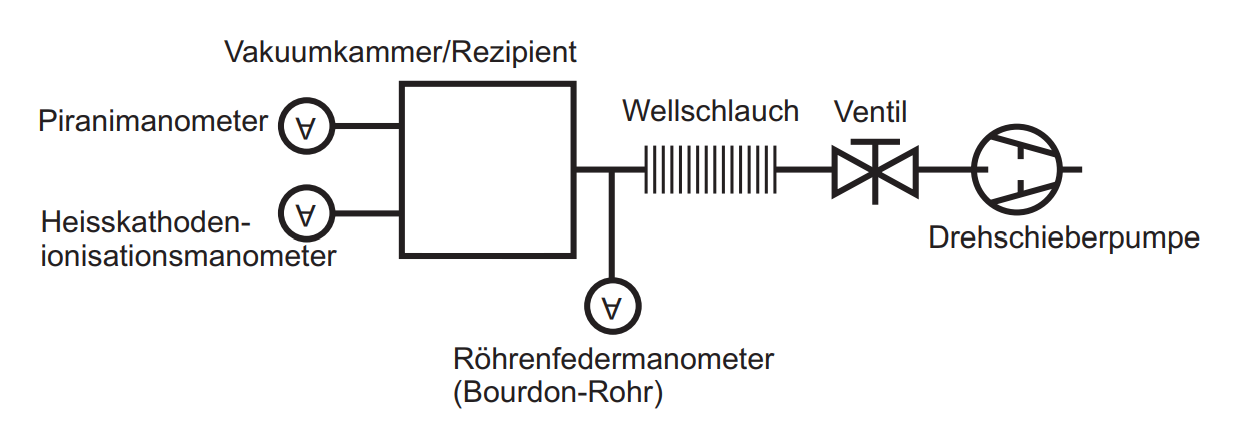
\includegraphics[width=.5\paperwidth]{aufbau21}
            \caption{generalisierter Aufbau zur Beobachtung der Funktionsweise einer Drehschieberpumpe}
            \label{fig:anord1}
        \end{figure}
    
    	
    	
    	Die Erwartung des von der Pumpe zu erzeugenden Vakuums beträgt
    	\begin{align*}
	    	P_E=5\cdot 10^{-2}\ mbar\\
	    	\Rightarrow \text{Schlussfolgerung: Leck}
    	\end{align*}
    	
    	
    	Messe Druck p  in der Vakuumkammer mit Dual Gauge Vakuumeter:
    	\begin{align*}
	    	\text{1. Lauf: }p=\cdot 10^{-1}\ mbar\\
	    	\text{2. Lauf: }p=\cdot 10^{-1}\ mbar
    	\end{align*}
    
    
    
    \subsection{Abpumpen kondensierbarer Dämpfe}
    
		\begin{figure}[H]
			\centering
			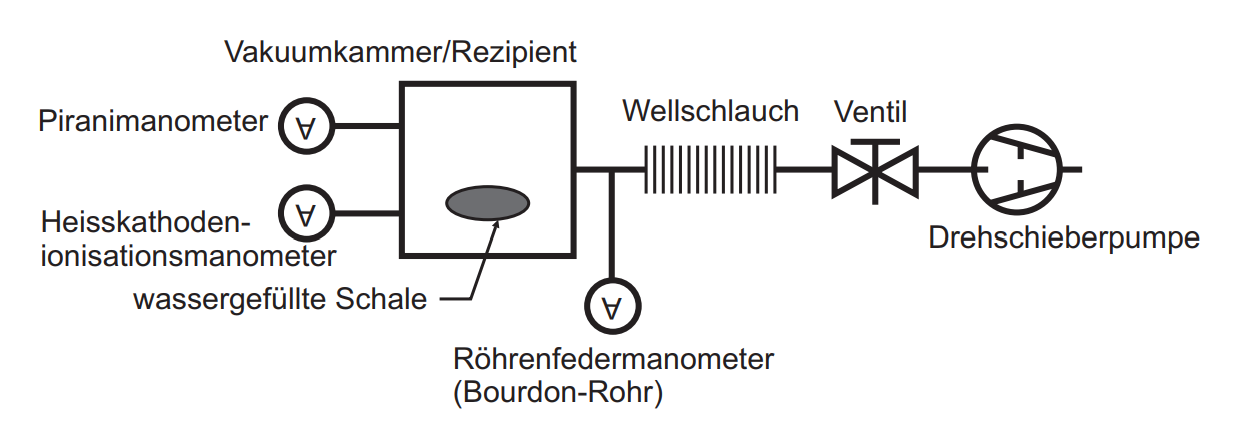
\includegraphics[width=.5\paperwidth]{aufbau22}
			\caption{Vakuum-Blockschaltbild zum Versuch des Abpumpens kondensierbarer Dämpfe}
            \label{fig:anord2}
		\end{figure}
	
		Beobachtung:
		\begin{itemize}
			\item Wasser beginnt bei niedrigem Druck an zu sieden ($-\ mbar$)
			
			$\rightarrow$ Schalte Gasballast zu um Kondensation des Wasserdampfes zu verhindern			
			
			\item Wasser gefriert bei $\ mbar$
			
		\end{itemize}

	
	\subsection{Inbetriebnahme einer Turbomolekularpumpe}
	
        \begin{figure}[H]
            \centering
            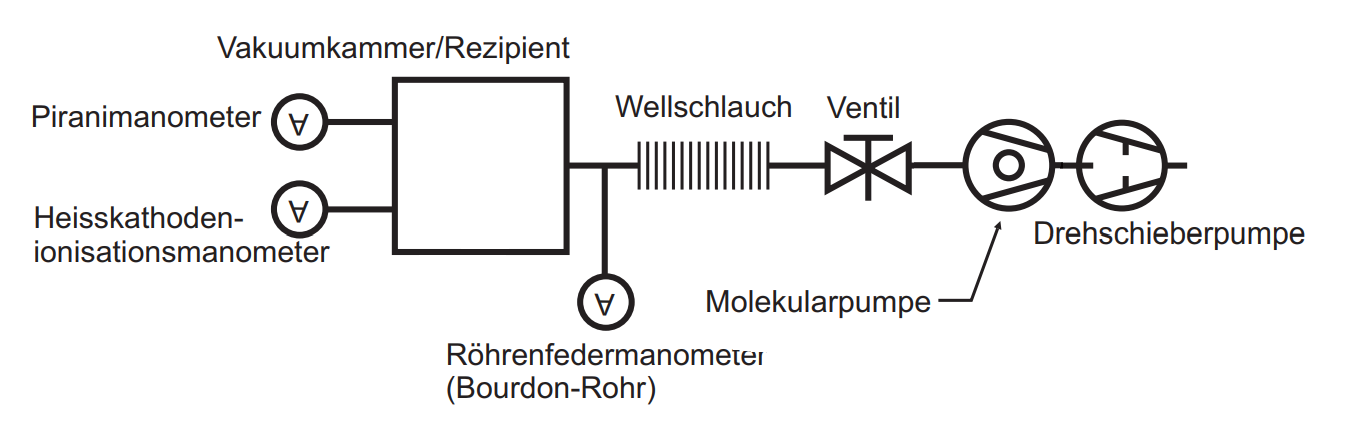
\includegraphics[width=.55\paperwidth]{aufbau23}
            \caption{Aufbau zur Beobachtung der Funktionsweise von Molekular- und Turbomolekularpumpe}
            \label{fig:anord3}
        \end{figure}
    
    	Die Turbomolekularpumpe wird nun nach \cite{skript}, wie in Aufbau \ref{fig:anord3} hinzugeschalten. Die Apparatur wurde eingeschaltet und über Nacht laufen gelassen.
    	
    	Über Nacht hat sich der Druck im Rezipienten auf $(\pm)\cdot 10^{-6}\ mbar$ eingestellt. (gemessen mit dem Dual-Gauge-Messgerät)
    
    
    \subsection{Saugvermögen der TMP}
    
        \begin{figure}[H]
            \centering
            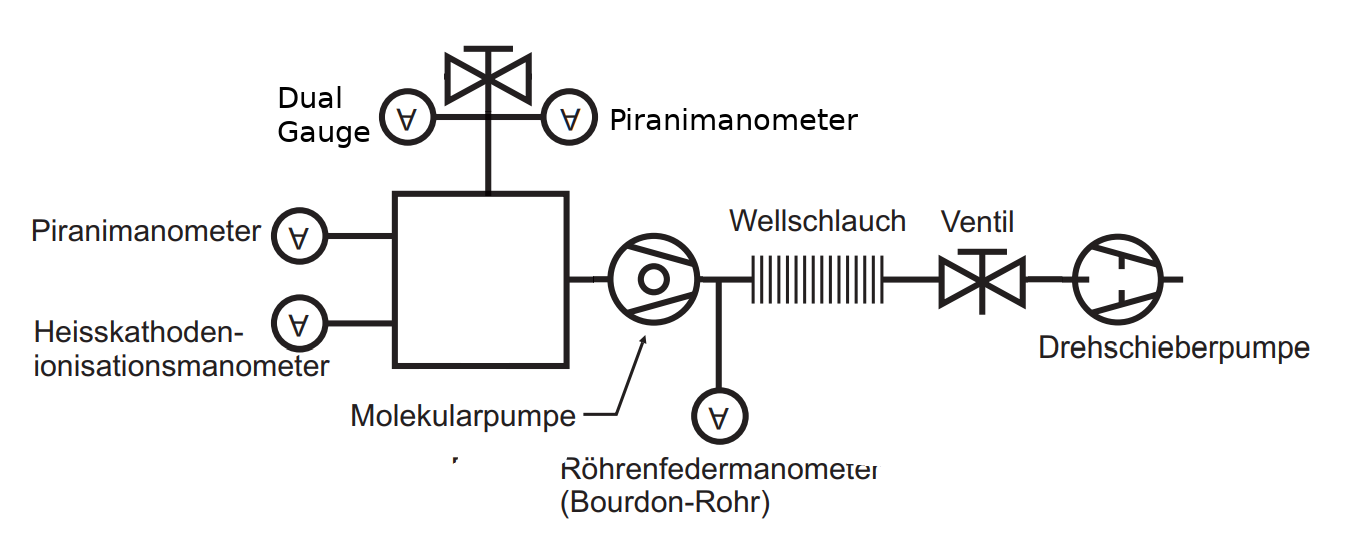
\includegraphics[width=.55\paperwidth]{aufbau24}
            \caption{Bestimmung des Saugvermögens einer TMP}
            \label{fig:anord4}
        \end{figure}
    
    	Es wird nun eine Kapillarröhre an den Rezipienten angeflanscht, diese hat ein Fassungsvolumen von $\ ml$
    
    	Mithilfe des Binärventils wird nun der gewünschte Druck eingestellt. Ein Seifentropfen wird in die Kapillare eingegeben und die Dauer gemessen, die der Tropfen benötigt um eine gewünschtes Volumen in der Kapillare zu überschreiten
    	
    	\begin{figure}[H]
    		\centering
    		\caption{Messreihe 1.1: Saugvermögen bei Kapillare 1}
    		\begin{tabular}{llll}
\toprule
                                   V / ml &                                     p / mbar &                                    t / s &                                       V / ml \\
\midrule
 $\left(1.00 \pm 0\right) \times 10^{-1}$ &  $\left(9.60 \pm 0.10\right) \times 10^{-6}$ &  $\left(3.31 \pm 0\right) \times 10^{1}$ &  $\left(3.00 \pm 0.10\right) \times 10^{-2}$ \\
 $\left(2.00 \pm 0\right) \times 10^{-1}$ &  $\left(2.90 \pm 0.10\right) \times 10^{-5}$ &  $\left(2.06 \pm 0\right) \times 10^{1}$ &  $\left(6.00 \pm 0.20\right) \times 10^{-2}$ \\
 $\left(2.00 \pm 0\right) \times 10^{-1}$ &  $\left(1.10 \pm 0.10\right) \times 10^{-4}$ &  $\left(5.73 \pm 0\right) \times 10^{0}$ &  $\left(6.00 \pm 0.20\right) \times 10^{-2}$ \\
 $\left(5.00 \pm 0\right) \times 10^{-1}$ &  $\left(2.90 \pm 0.10\right) \times 10^{-4}$ &  $\left(1.25 \pm 0\right) \times 10^{1}$ &  $\left(3.00 \pm 0.10\right) \times 10^{-1}$ \\
  $\left(1.00 \pm 0\right) \times 10^{0}$ &  $\left(1.10 \pm 0.10\right) \times 10^{-3}$ &  $\left(4.54 \pm 0\right) \times 10^{0}$ &  $\left(4.00 \pm 0.10\right) \times 10^{-1}$ \\
\bottomrule
\end{tabular}

    	\end{figure}
    	
    	Die Kapillare wurde nun durch eine Andere ersetzte, diese besitzt ein Fassungsvolumen von $\ ml$, und es wurden folgende Messungen gemacht:
    	
 	    \begin{figure}[H]
    		\centering
    		\caption{Messreihe 1.2: Saugvermögen bei Kapillare 2}
    		%TODO:  \begin{tabular}{lll}
\toprule
                                    p / mbar &                                    t / s &                                      V / ml \\
\midrule
 $\left(1.10 \pm 0.10\right) \times 10^{-3}$ &  $\left(5.45 \pm 0\right) \times 10^{1}$ &  $\left(5.00 \pm 0.50\right) \times 10^{0}$ \\
 $\left(2.90 \pm 0.10\right) \times 10^{-4}$ &  $\left(6.10 \pm 0\right) \times 10^{1}$ &  $\left(2.00 \pm 0.50\right) \times 10^{0}$ \\
 $\left(3.10 \pm 0.10\right) \times 10^{-3}$ &  $\left(2.40 \pm 0\right) \times 10^{1}$ &  $\left(5.50 \pm 0.50\right) \times 10^{0}$ \\
 $\left(1.00 \pm 0.10\right) \times 10^{-2}$ &  $\left(1.71 \pm 0\right) \times 10^{1}$ &  $\left(1.00 \pm 0.05\right) \times 10^{1}$ \\
 $\left(3.40 \pm 0.10\right) \times 10^{-2}$ &  $\left(1.13 \pm 0\right) \times 10^{1}$ &  $\left(1.50 \pm 0.05\right) \times 10^{1}$ \\
\bottomrule
\end{tabular}

    	\end{figure}
    	
    	Es erfolgt eine weitere Kapillare mit dem Fassungsvermögen von $\ ml$, mit den folgenden Messungen:
    	
    	\begin{figure}[H]
			\centering
			\caption{Messreihe 1.3: Saugvermögen bei Kapillare 3}
			%TODO:  \begin{tabular}{llll}
\toprule
Empty DataFrame
Columns: Index(['p / mbar', 't / s', 'V / ml'], dtype='object')
Index: RangeIndex(start=0, stop=0, step=1) \\
\bottomrule
\end{tabular}

		\end{figure}
    	
    	Zuletzt wird ein Kolben angebracht:
    	
    	\begin{itemize}
    		\item Gesamtvolumen: $\ ml$
    		\item Masse: $m=(\pm)\ g$
    		\item Skalenteilung: $\ ml$
    		\item Durchmesser: $d=(\pm)\cdot10^{-2}\ m$
    	\end{itemize}
    
    	\begin{figure}[H]
			\centering
			\caption{Messreihe 1.4: Saugvermögen bei Kolben}
			%TODO:  \begin{tabular}{llll}
\toprule
Empty DataFrame
Columns: Index(['p / mbar', 't / s', 'V / ml'], dtype='object')
Index: RangeIndex(start=0, stop=0, step=1) \\
\bottomrule
\end{tabular}

		\end{figure}
    	
    	(Diese Messungen geschehen bei Äußerem Normaldruck)
    	Anschließend wird langsam belüftet um die TMP nicht zu überhitzen
    	
    
    \subsection{Leitwert von Rohr und Blende}
    
        \begin{figure}[H]
            \centering
            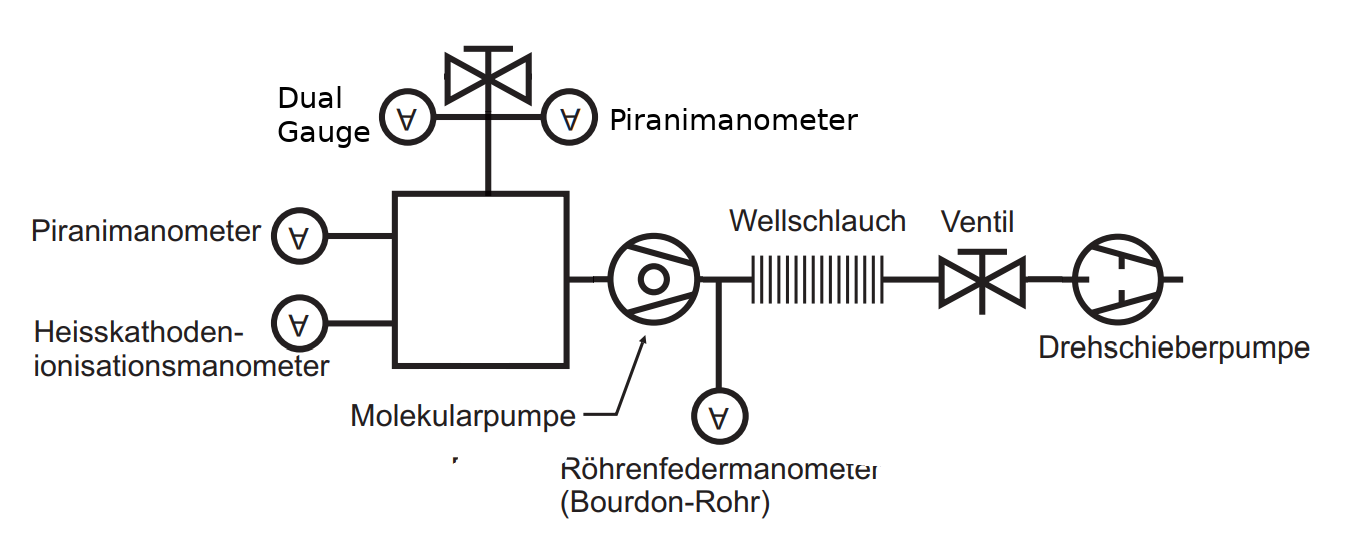
\includegraphics[width=.55\paperwidth]{aufbau24.png}
            \caption{Aufbau zur Bestimmung des Leitwerts von Rohr und Blende}
            \label{fig:anord5}
        \end{figure}
    
    	Der Rezipient wird nun leer gepumpt und anschließend mittels Binärventil der gewünschte Druck eingestellt. Bei verschiedenen Rohren und Blenden in der Führung wird der Druck jeweils oben am Führrohr und unten am Rezipienten gemessen (mithilfe der Dual-Gauge)
    	
    	\begin{itemize}
    		\item Maße Blende:
    			\begin{align*}
    				d=&(\pm)\cdot 10^{-2}\ m\\
    				h=&(\pm)\cdot 10^{-2}\ m
    			\end{align*}
    			
    		\item Maße Rohr:
    			\begin{align*}
    				d=&(\pm)\cdot 10^{-2}\ m\\
    				h=&(\pm)\cdot 10^{-2}\ m
    			\end{align*}
    			
    		\item Maße Halterohr:
    			\begin{align*}
    				d=&(\pm)\cdot 10^{-2}\ m\\
    				h=&(\pm)\cdot 10^{-2}\ m
    			\end{align*}
    	\end{itemize}
    
    	\begin{figure}[H]
    		\centering
    		\caption{Messreihe 2.1: Rohr und Blende}
    		%TODO: \begin{tabular}{ll}
\toprule
                                $p_o$ / mbar &                                 $p_u$ / mbar \\
\midrule
 $\left(5.80 \pm 0.10\right) \times 10^{-3}$ &  $\left(5.40 \pm 0.10\right) \times 10^{-5}$ \\
 $\left(2.40 \pm 0.10\right) \times 10^{-2}$ &  $\left(9.70 \pm 0.10\right) \times 10^{-5}$ \\
 $\left(4.40 \pm 0.10\right) \times 10^{-2}$ &  $\left(1.70 \pm 0.10\right) \times 10^{-4}$ \\
 $\left(7.10 \pm 0.10\right) \times 10^{-2}$ &  $\left(3.30 \pm 0.10\right) \times 10^{-4}$ \\
 $\left(9.50 \pm 0.10\right) \times 10^{-2}$ &  $\left(5.60 \pm 0.10\right) \times 10^{-4}$ \\
 $\left(1.30 \pm 0.10\right) \times 10^{-1}$ &  $\left(1.10 \pm 0.10\right) \times 10^{-3}$ \\
 $\left(1.80 \pm 0.10\right) \times 10^{-1}$ &  $\left(2.00 \pm 0.10\right) \times 10^{-3}$ \\
 $\left(2.20 \pm 0.10\right) \times 10^{-1}$ &  $\left(3.30 \pm 0.10\right) \times 10^{-3}$ \\
 $\left(2.60 \pm 0.10\right) \times 10^{-1}$ &  $\left(5.70 \pm 0.10\right) \times 10^{-3}$ \\
 $\left(3.20 \pm 0.10\right) \times 10^{-1}$ &  $\left(1.00 \pm 0.10\right) \times 10^{-2}$ \\
\bottomrule
\end{tabular}

   		\end{figure}
   	
   		Nach der Messung wird die Pumpe belüftet. Das Halterohr abgeschraubt und die Blende entfernt. Nach erneutem anbringen des Halterohrs wird erneut eine Druckmessung durchgeführt.
   	
   		\begin{figure}[H]
   			\centering
   			\caption{Messreihe 2.2: Rohr}
   			%TODO: \begin{tabular}{ll}
\toprule
                                $p_o$ / mbar &                                 $p_u$ / mbar \\
\midrule
 $\left(5.90 \pm 0.10\right) \times 10^{-3}$ &  $\left(5.50 \pm 0.10\right) \times 10^{-5}$ \\
 $\left(2.20 \pm 0.10\right) \times 10^{-2}$ &  $\left(1.00 \pm 0.10\right) \times 10^{-4}$ \\
 $\left(4.20 \pm 0.10\right) \times 10^{-2}$ &  $\left(1.80 \pm 0.10\right) \times 10^{-4}$ \\
 $\left(6.60 \pm 0.10\right) \times 10^{-2}$ &  $\left(3.40 \pm 0.10\right) \times 10^{-4}$ \\
 $\left(8.70 \pm 0.10\right) \times 10^{-2}$ &  $\left(5.50 \pm 0.10\right) \times 10^{-4}$ \\
 $\left(1.20 \pm 0.10\right) \times 10^{-1}$ &  $\left(1.00 \pm 0.10\right) \times 10^{-3}$ \\
 $\left(1.50 \pm 0.10\right) \times 10^{-1}$ &  $\left(1.80 \pm 0.10\right) \times 10^{-3}$ \\
 $\left(2.00 \pm 0.10\right) \times 10^{-1}$ &  $\left(3.20 \pm 0.10\right) \times 10^{-3}$ \\
 $\left(2.40 \pm 0.10\right) \times 10^{-1}$ &  $\left(5.60 \pm 0.10\right) \times 10^{-3}$ \\
 $\left(3.10 \pm 0.10\right) \times 10^{-1}$ &  $\left(1.10 \pm 0.10\right) \times 10^{-2}$ \\
\bottomrule
\end{tabular}

   		\end{figure}
   	
   		Die Pumpe wird belüftet und als letzte Messreihe lediglich die Blende in das Halterohr montiert. Der Rezipient wird erneut evakuiert und eine erneute Druckmessung durchgeführt.
   	
   		\begin{figure}[H]
   			\centering
   			\caption{Messreihe 2.3: Blende}
   			%TODO: \begin{tabular}{ll}
\toprule
                                $p_o$ / mbar &                                 $p_u$ / mbar \\
\midrule
 $\left(9.40 \pm 0.10\right) \times 10^{-4}$ &  $\left(5.60 \pm 0.10\right) \times 10^{-5}$ \\
 $\left(3.20 \pm 0.10\right) \times 10^{-3}$ &  $\left(9.80 \pm 0.10\right) \times 10^{-5}$ \\
 $\left(7.30 \pm 0.10\right) \times 10^{-3}$ &  $\left(1.80 \pm 0.10\right) \times 10^{-4}$ \\
 $\left(1.40 \pm 0.10\right) \times 10^{-2}$ &  $\left(3.20 \pm 0.10\right) \times 10^{-4}$ \\
 $\left(2.40 \pm 0.10\right) \times 10^{-2}$ &  $\left(5.60 \pm 0.10\right) \times 10^{-4}$ \\
 $\left(4.10 \pm 0.10\right) \times 10^{-2}$ &  $\left(1.00 \pm 0.10\right) \times 10^{-3}$ \\
 $\left(6.20 \pm 0.10\right) \times 10^{-2}$ &  $\left(1.90 \pm 0.10\right) \times 10^{-3}$ \\
 $\left(9.10 \pm 0.10\right) \times 10^{-2}$ &  $\left(3.30 \pm 0.10\right) \times 10^{-3}$ \\
 $\left(1.20 \pm 0.10\right) \times 10^{-1}$ &  $\left(5.40 \pm 0.10\right) \times 10^{-3}$ \\
 $\left(1.70 \pm 0.10\right) \times 10^{-1}$ &  $\left(1.00 \pm 0.10\right) \times 10^{-2}$ \\
\bottomrule
\end{tabular}

   		\end{figure}    
    
    
    \subsection{Lecksuche}
    
		Zunächst wird der Aufbau aus Versuchsteilen 4 \& 5 benutzt\\\\	
		$\rightarrow$ Über Nacht hat sich ein Druck von $(\pm)\cdot 10^{}\ mbar$ eingestellt.\\\\
		Die Pumpen werden erneut eingeschalten. Es wird ein aus Glas geschmolzenes Leck aus dem Auslass des Ventils am Rezipienten angebracht.\\
		$\rightarrow$ Mit dem Leck stellt sich ein Druck von $(\pm)\cdot 10^{}\ mbar$ ein.\\		
		Die Strahlenkanone wurde dann auf die Glaskapillare gehalten.\\
		$\rightarrow$ Der Luftstrom war durch die Gasentladung sehr deutlich zu sehen.\\\\		
		Für die Gegenstromlecksuche wurde folgender Aufbau verwendet:
		
		\begin{figure}[H]
			\centering
			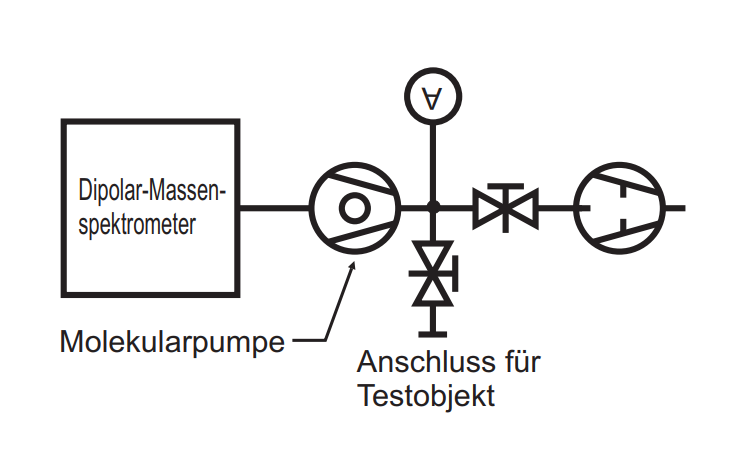
\includegraphics[width=.3\paperwidth]{aufbau262}
			\caption{Prinzipschaltbild des im Versuchsteil 6 eingesetzten Gegenstromlecksuchers}
			\label{fig:anord6}
		\end{figure}
		Mittels einer Heliumgasflasche wurde am verschiedenen Stellen Helium auf die Apparatur gegeben und der Ausschlag am Spektrometer beobachtet.\\
		$\rightarrow$ Es konnte eine poröse Schweißnaht ausfindig gemacht werden, die offensichtlich für das Leck im Aufbau verantwortlich ist.

	\section{Ergebnisse}
	\subsection{Inbetriebnahme der Drehschieberpumpe}
	
		Nach Inbetriebnahme der Drehschieberpumpe wurde der Druck im Rezipienten mittels des Dual-Gauge-Druckmessgerätes verfolgt.
		
		Nach kurzer Laufzeit der Pumpe wird die Druckveränderung mitverfolgt, dabei fällt der Druck innerhalb von $\ min$ von $(\pm)\cdot 10^{-2}\ mbar$ auf $(\pm)\cdot 10^{-2}\ mbar$ ab. Aufgrund der Geschwindigkeit dieses Abfalls schätzen wir, dass der Druck nicht unter einen Wert von
		
		\begin{align}
			p=(\pm)\cdot 10^{-2}\ mbar
		\end{align}
		
		(Fehler ist Schätzung) fallen wird, auch wenn wir die Pumpe über mehrere Stunden Hinweg arbeiten lassen könnten.
		
		Das Vakuum kann mit einer Drehschieberpumpe nicht beliebig gut werden, da die Drehschieberpumpe bei einem gewissen Druck das Gas nicht mehr genügend komprimieren kann, was zuum Ausstoßen des Gases nötig wäre. 
		Es stellt sich aber ein Gleichgewicht bei einem bestimmten Druck ein, sodass die Menge an Gas, die von der Pumpe nach außen gefördert wird, gerade der Menge Gas entspricht, die durch Lecks in den Rezipienten eintritt.
		
		
	\subsection{Abpumpen kondensierbarer Dämpfe}
		
		\begin{figure}[H]
			\centering
			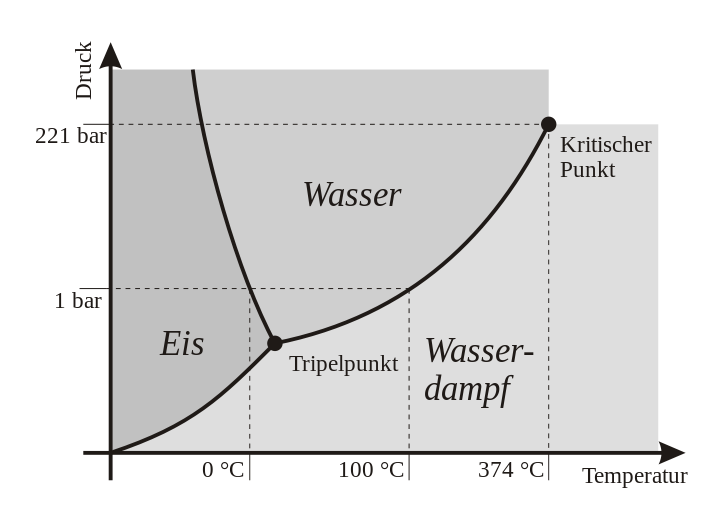
\includegraphics[width=.5\paperwidth]{phasen-wasser}
			\caption{Phasendiagramm von Wasser (nach \cite{wikibooks})}
		\end{figure}
	
	% continuation: 47727...
	
	\section{Diskussion}
	
	Hier werden alle wesentlichen Ergebnisse nochmals ausgefuehrt und diskutiert. 
	
	Am Schluss kann man noch eine allgemeinere Bemerkung zum Versuch machen.
	
	
	\newpage 
	
	\begin{thebibliography}{00}   % {00}: max 2-stellig
		
		\bibitem{skript} Versuchsskript zu Versuch F70
		
		\bibitem{wikibooks} de.wikibooks.org: Aggregatszustandsänderungen\\ (\url{https://de.wikibooks.org/wiki/Physik_in_unserem_Leben/_Aggregatzustands%C3%A4nderungen})
		
	\end{thebibliography}
	
\end{document}